\section{Principal Component Analysis}
\label{DatabehandlingPCA}
%
Først laves en \textit{Principal Component Analysis} (PCA) analyse på det samlede datasæt, for at undersøge om der er korrelation mellem nogle af de 23 skala spørgsmål. For at undersøge hvor meget af variansen, der kan forklares ud fra hver \textit{Principal Components} (PC) udarbejdes der et \textit{Scree}-plot, jævnfør \autoref{fig:Scree}. 
%
\begin{figure}[H]
\centering
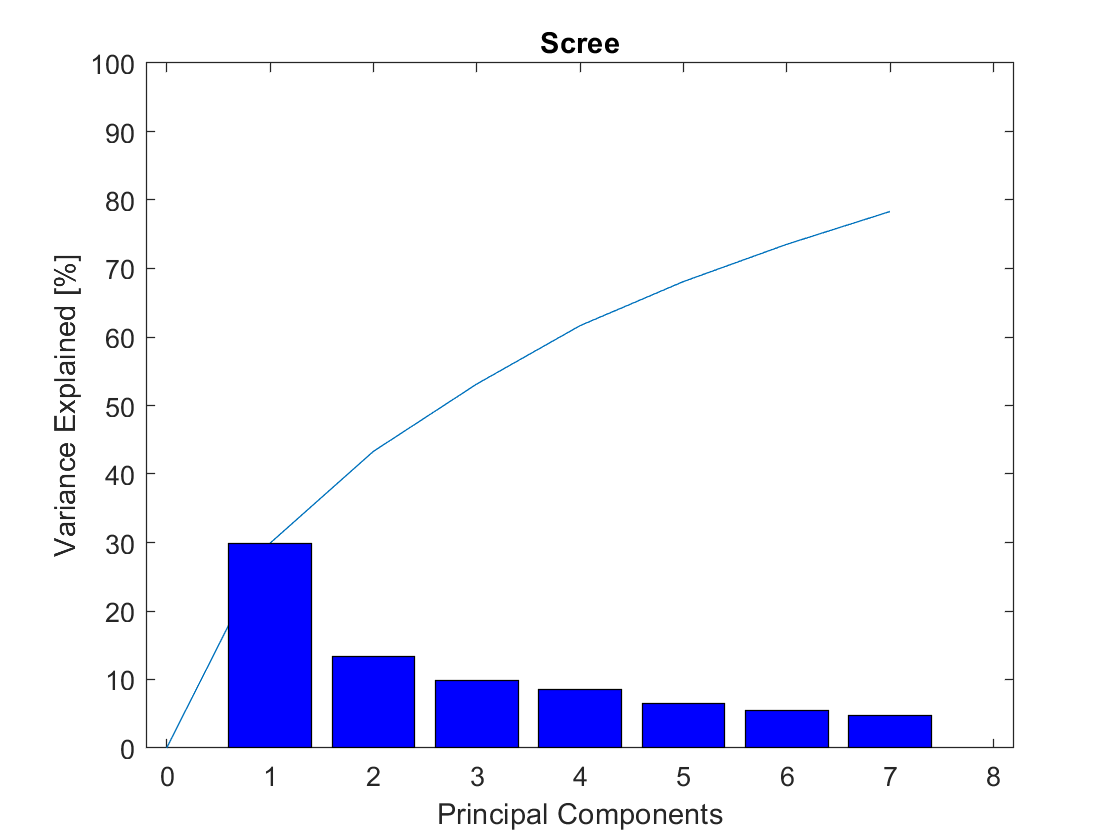
\includegraphics[width=\textwidth]{Figure/DatabehandlingSkalaer/PCAfigures/Scree.png}
\caption{\textit{Scree}-plot, hvorpå sammenhængen mellem antallet af \textit{Principal Components} og \textit{Variance Explained [\%]} fremgår.}
\label{fig:Scree}
\end{figure}
\noindent
%
Ud fra \textit{Scree}-plottet på \autoref{fig:Scree} fremgår det, at der ikke er en tydelig sammenhæng i variansen fra datasættet, da kun 29.9 \% af variansen kan forklares af PC1 og 13.4 \% af PC2. Selv hvis de tre første PCs medtages, er det kun 53.1 \% af variansen, som forklares af modellen. Dette skyldes formentligt, at der er for mange variable, som bliver varieret på én gang og at det ikke har været muligt at kontrollere alle variable lige godt, og at der tilmed forekommer forskellige grupperinger i forhold til de variable, der tilnærmelsesvist var mulige at kontrollere. På baggrund af det er det svært at vurdere hvilke parametre, der korrelerer.\blankline 
%
Ud fra \textit{Score}-plottet på \autoref{fig:Score} fremgår det også at PC1 kun forklarer en lille del af variansen, da der er meget spredning i datapunkterne og spredningen ikke er systematisk. Hvis PC1 havde forklaret en større del af variansen, ville data være mere centreret omkring den horisontale akse.
%
\begin{figure}[H]
\centering
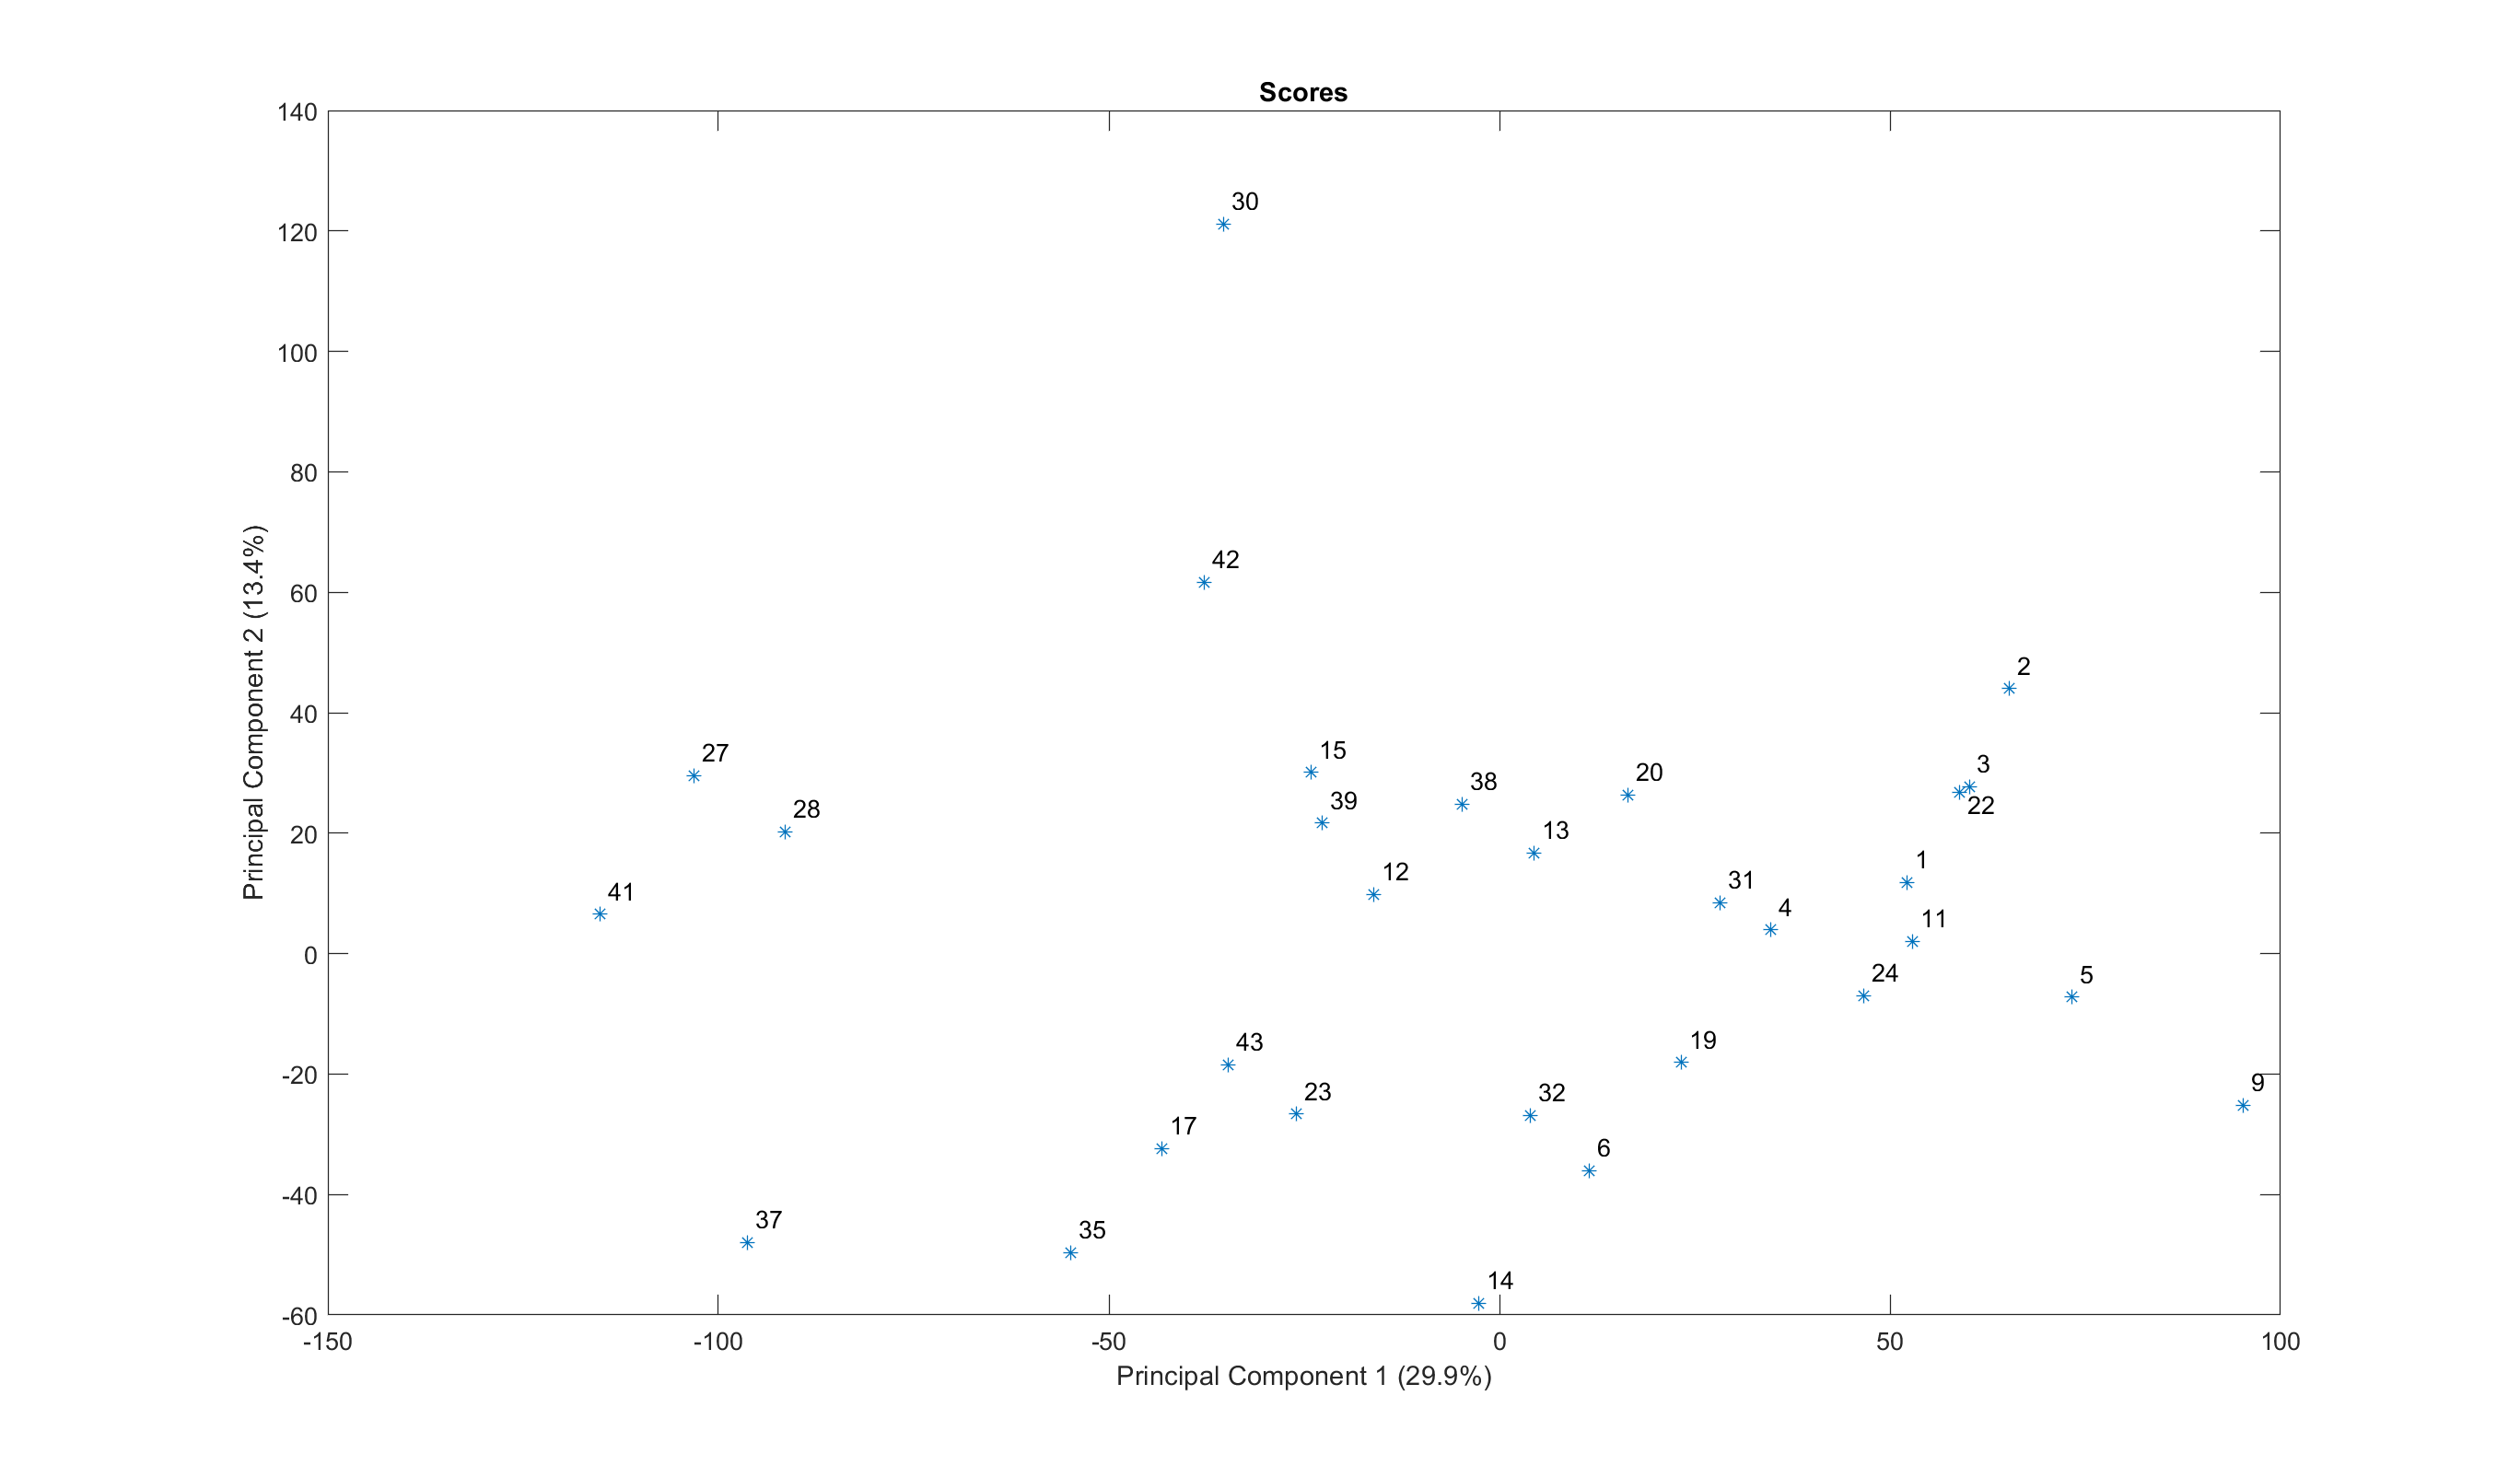
\includegraphics[width=\textwidth]{Figure/DatabehandlingSkalaer/PCAfigures/Scores}
\caption{\textit{Score}-plot for PC1 og PC2.}
\label{fig:Score}
\end{figure}
\noindent
%
For at undersøge hvilke parametre, der bidrager til hver PC opstilles et \textit{Bi}-plot, hvori både \textit{scores} og \textit{loadings} fremgår. \textit{Bi}-plottet på \autoref{fig:Biplot} giver det bedste overblik, da det er nemmest at fortolke i to dimensioner, dog er det tredimensionelle plot vedlagt i \fullref{ElektroniskBilag3D}. 
%
\begin{figure}[H]
\centering
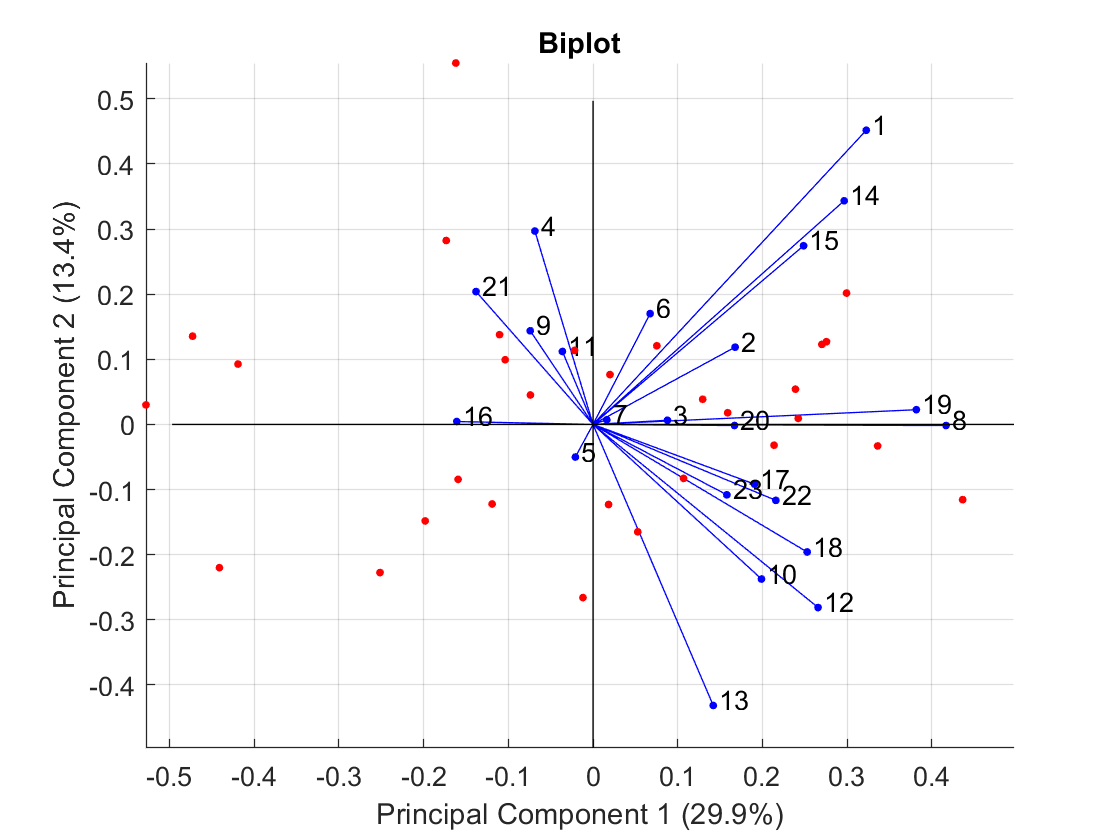
\includegraphics[width=\textwidth]{Figure/DatabehandlingSkalaer/PCAfigures/Biplot}
\caption{\textit{Bi}-plot med både \textit{loadings} (angivet med blå) og \textit{scores} (angivet med rød) fremgår i forhold til robottens højde.}
\label{fig:Biplot}
\end{figure}
\noindent
%
Baseret på \autoref{fig:Biplot} tyder det på, at der forekommer en positiv korrelation mellem SQ14, vedrørende hvor personlig robottens hjælp opleves, og SQ15, vedrørende hvor overrasket testpersonerne blev over robottens henvendelse. Lignende korrelation forefindes mellem SQ17, vedrørende hvor elegant robotten opleves, og SQ22, vedrørende hvor sjov robotten opleves. Derudover tyder det på, at der forekommer en positiv korrelation mellem SQ8, vedrørende hvorvidt testpersonerne føler, at robotten kan hjælpe dem, SQ19, vedrørende hvor sød robotten opleves, og SQ20, vedrørende hvor sej robotten opleves. De tre parametre tyder på at være negativ korrelerede med SQ16, vedrørende hvor irriterende robotten opleves. En negativ korrelation forefindes også mellem SQ4, vedrørende hvordan robottens bevægelser opleves, og SQ13, vedrørende hvorvidt testpersonerne regnede med at robotten fulgte dem hen til det valgte sted. 

Baseret på \autoref{fig:Biplot} fremgår det, at SQ7, vedrørende robottens højde, SQ5, vedrørende robottens afstand, og SQ3, vedrørende hvordan det var at bruge robotten, kun forklare en meget lille del af variationen. Tages der i 3D plottet udgangspunkt i SQ7, fremgår det ligeledes at denne parametre ikke bidrager med noget til de tre PCs. Sammenholdes det med hvad der er beskrevet i \fullref{TestAfSkalaVarians} på \autoref{fig:Varians}, hvor det fremgår at SQ7 har en meget lille varians, så er det ikke overraskende, at den ikke bidrager mere til de tre PCs end den gør. Dette afspejler at testpersonerne har svaret nogenlunde det samme til SQ7, det kan derfor tyde på at SQ7 ikke er særlig vigtig for den samlede brugeroplevelse. At SQ7 kun forklarer en meget lille del af variationen kan skyldes flere ting; enten så er robottens højde ikke en vigtig parameter eller så er testpersonerne ikke blevet eksponeret for en højde, der reelt påvirker deres oplevelse. Det kan også være fordi, at SQ7 bliver målt indirekte i andre parametre, som netop påvirkes af robottens højde, hvorfor dette vil blive undersøgt nærmere i det følgende afsnit.\blankline
%
Ud fra resultaterne fra denne PCA kan der ikke drages nogle særlig håndgribelige konklusioner i forhold til hvilke parametre korrelere positiv eller negativt, eller slet ikke. For at undersøge om der er nogle tendenser i forhold til de objektive parametre, som blev justeret undervejs i testen; højde, afstand samt robottens indgangsvinkel, vil hver af disse parametre blive undersøgt med en PCA. Dette gøres ved at fokusere på et af de tre objektive parametre ad gangen og dele data op i de grupper, som allerede findes.




